% SPDX-License-Identifier: Apache-2.0
%
% FireSim over Ethernet on the AX7A200B. Built by //docs:firesim. Every
% listing is included from the tree; every number is from a build or a
% board run, with its date.
\documentclass[journal,9pt]{IEEEtran}

% Listings of Rust set by rustfmt at 80 columns: 5.6pt is what fits
% the frame of a column (issue 1061).
\newcommand{\listingsize}{\fontsize{5.6}{6.6}\selectfont}
% SPDX-License-Identifier: Apache-2.0
%
% The house preamble, shared by every document in this directory. Loaded
% after \documentclass, before \title. Keeping it in one file is what
% stops two articles drifting apart in font, listing style or figure
% style.
% Computer Modern. IEEEtran selects Times (ptm) by default, so the face has
% to be chosen explicitly.
%
% Latin Modern is the Computer Modern variety used here, and the choice is
% forced rather than aesthetic. Under T1 encoding, plain `cmr` has no Type 1
% outlines unless cm-super is installed, and it is not in the pinned
% distribution, so pdflatex falls back to EC bitmaps and every glyph in the
% PDF becomes a Type 3 font. That was measured: the first build produced a
% document with 10 Type 3 fonts and no Type 1. Latin Modern is Computer
% Modern redrawn with a full T1 repertoire and real .pfb outlines, so the
% same design comes out scalable.
\usepackage[T1]{fontenc}
\usepackage[utf8]{inputenc}
\usepackage{lmodern}
% microtype is not in the pinned TeX distribution. emergencystretch alone
% keeps the two-column measure from producing overfull lines.
\setlength{\emergencystretch}{3em}

\usepackage{amsmath}
\usepackage{amssymb}
\usepackage{amsthm}
\usepackage{booktabs}
\usepackage{array}
% enumitem is not in the pinned TeX distribution; the list spacing below
% does what \setlist would have done.
\usepackage{float}
\usepackage{xcolor}
\usepackage{listings}
\usepackage{tikz}
\usetikzlibrary{arrows.meta,positioning,fit,backgrounds,calc}
\usepackage[hidelinks,bookmarks=true]{hyperref}

% Numbered, definition-style box for a rule the reader is meant to apply.
\theoremstyle{definition}
\newtheorem{rulebox}{Rule}
\newtheorem{example}{Example}

% Unnumbered asides.
\theoremstyle{remark}
\newtheorem*{tip}{Tip}
\newtheorem*{pitfall}{Pitfall}

% Tighter lists, in place of enumitem's \setlist.
\setlength{\topsep}{2pt}
\setlength{\itemsep}{1pt}
\setlength{\parsep}{0pt}

% Code in the running text. The typewriter face under T1 ligates `<<`
% and `>>` into guillemets, so a shift printed as \code{<<} came out as
% a French quotation mark (issue 571). microtype's \DisableLigatures is
% not in the pinned distribution, but the primitive it rests on is
% pdfTeX's own: \pdfnoligatures strips every ligature from the font it
% is given, and the current font inside \texttt is the typewriter face
% at the size in use, so each size is stripped the first time \code
% sets it. Code wants no ligature at all: two quotes are two quotes.
\newcommand{\code}[1]{\texttt{\ifdefined\pdfnoligatures\pdfnoligatures\font\fi #1}}
\newcommand{\term}[1]{\emph{#1}}

% Syntax highlighting. Four roles, distinguishable in colour and still
% distinguishable in greyscale, because an IEEE article gets printed: the
% keyword is the only bold role, the comment is the only italic one, and the
% two remaining roles differ in lightness as well as in hue.
\definecolor{kwblue}{RGB}{20,60,150}
\definecolor{cmtgreen}{RGB}{90,120,90}
\definecolor{strred}{RGB}{150,50,40}
\definecolor{numgray}{gray}{0.45}
\definecolor{framegray}{gray}{0.70}
\definecolor{bgshade}{gray}{0.97}
% A darker fill for figure cells. The listing background has to stay very
% light to keep code readable; a figure cell has to be clearly shaded or the
% distinction it draws is invisible in print.
\definecolor{cellshade}{gray}{0.90}

% The listing size is the document's choice, because it depends on the
% column: a two-column article sets `\listingsize` to 6pt and keeps its
% listings within 70 columns, or to 5.6pt when it includes source that
% rustfmt sets at 80, which is what fits a column's frame (issue 1061);
% a one-column document keeps the body size and includes source files
% at 80. `//docs:frame_test` checks every listing line against its frame. Lines are never broken; a line that does not fit
% overflows the frame, which is visible, rather than wrapping, which is
% not.
\providecommand{\listingsize}{\scriptsize}

% `'` is deliberately not a string delimiter: the language uses it for loop
% labels, as Rust does, so treating it as a quote would swallow the rest of
% the line.
\lstdefinestyle{txhdl}{
  basicstyle=\ttfamily\listingsize,
  keywordstyle=\bfseries\color{kwblue},
  commentstyle=\itshape\color{cmtgreen},
  stringstyle=\color{strred},
  numberstyle=\tiny\color{numgray},
  morekeywords={mod,use,pub,const,type,struct,enum,trait,impl,fn,async,let,mut,
    match,if,else,loop,while,for,in,break,continue,return,as,await,
    module,bus,channel,transaction,protocol,pipeline,flow,seq,config,
    port,stage,pipe,instance,connect,bind,tag,domain,blackbox,foreign,
    property,role,signal,handler,true,false,
    sequence,interface,modport,implements,package,import,var,wire,func,proc,
    case,default,next,fork,branch,join,state,fsm},
  morecomment=[l]{//},
  morestring=[b]",
  showstringspaces=false,
  columns=fullflexible,
  keepspaces=true,
  breaklines=false,
  % Framed, so a listing is bounded rather than floating in the column.
  frame=single,
  rulecolor=\color{framegray},
  framesep=3pt,
  backgroundcolor=\color{bgshade},
  xleftmargin=3pt,
  xrightmargin=3pt,
  aboveskip=6pt,
  belowskip=6pt,
  % Every listing is numbered and captioned, so it can be referred to by
  % number. `caption` without `float` numbers the listing and leaves it
  % where it was written, which is what a listing in running prose needs.
  captionpos=b,
  abovecaptionskip=2pt,
  belowcaptionskip=6pt,
}

% Figures drawn as text. Framed the same way, and with the highlighting
% switched off, because a box-and-arrow diagram is not code and half its
% words turning blue reads as an accident. Setting a style adds keys rather
% than clearing the ones already set, so the three roles are neutralised by
% hand rather than by leaving them out. Program output is printed in this
% style too, and a netlist's assignment can run past the frame, so a line
% that does not fit is broken and the rest indented; source never is.
\lstdefinestyle{ascii}{
  basicstyle=\ttfamily\listingsize,
  keywordstyle=\ttfamily,
  commentstyle=\ttfamily,
  stringstyle=\ttfamily,
  columns=fullflexible,
  keepspaces=true,
  breaklines=true,
  breakindent=2em,
  frame=single,
  rulecolor=\color{framegray},
  framesep=3pt,
  backgroundcolor=\color{bgshade},
  xleftmargin=3pt,
  xrightmargin=3pt,
  aboveskip=6pt,
  belowskip=6pt,
}
\lstset{style=txhdl}

% House TikZ styles. `shorten` lives on the arrow styles rather than on each
% arrow, so every arrow in the document gets the gap, including ones added
% later. TikZ clips a path at a node's border, so without it an arrowhead
% butts against the box with no gap at all. Keep `node distance` well above
% twice the shorten, or the arrow shrinks to nothing.
\tikzset{
  box/.style={draw,rounded corners=2pt,align=center,inner sep=4pt,
              font=\footnotesize},
  boxf/.style={box,fill=bgshade},
  lbl/.style={font=\scriptsize\itshape,align=center},
  fl/.style={-{Stealth[length=4pt]},shorten >=2.5pt,shorten <=2.5pt},
  fld/.style={fl,dashed},
}


% The contents list: the class gives a section's number 2.75em, which
% a Roman numeral past thirty overruns onto the title, so the box is
% wider here, and a subsection's entry starts where a title does.
\makeatletter
\def\l@section#1#2{\addpenalty{\@secpenalty}\addvspace{1.0em plus 1pt}%
    \@tempdima 5.75em \begingroup \parindent \z@ \rightskip \@pnumwidth%
    \parfillskip-\@pnumwidth {\bfseries\leavevmode #1}\hfil\hbox to\@pnumwidth{\hss #2}\par%
    \endgroup}
\def\l@subsection{\@dottedtocline{2}{5.75em}{5em}}
\def\l@subsubsection{\@dottedtocline{3}{10.75em}{5.5em}}
\makeatother


\InputIfFileExists{buildstamp.tex}{}{}
\providecommand{\buildstamp}{Draft build (outside the Bazel flow).}

% A range of the stream part, by its begin/end markers.
\newcommand{\streampart}[3]{%
\lstinputlisting[rangebeginprefix=//\ begin\{,rangebeginsuffix=\},%
rangeendprefix=//\ end\{,rangeendsuffix=\},includerangemarker=false,%
linerange=#1-#1,caption={#2},label={#3}]{lib/parts/src/remote/stream.rs}}

\definecolor{tint}{RGB}{232,238,250}
\tikzset{
  box/.style={draw, rounded corners=2pt, minimum height=5mm, inner sep=2pt, align=center, font=\scriptsize},
  art/.style={draw, fill=tint, rounded corners=2pt, minimum height=5mm, inner sep=2pt, align=center, font=\scriptsize},
  flow/.style={-{Stealth[length=1.6mm]}, thick},
  both/.style={{Stealth[length=1.6mm]}-{Stealth[length=1.6mm]}, thick},
  lbl/.style={font=\tiny, fill=white, inner sep=1pt},
}

\title{FireSim over Ethernet:\\A Rocket Core on a Low-Cost FPGA Board}

\author{Filip Filmar and Dragiša Janković%
\thanks{Both authors are independent. Filip Filmar is the
corresponding author, at f@hdlfactory.com; Dragiša Janković is
reached at linkedin.com/in/dragisa-jankovic.}%
\thanks{This document reports FireSim run on the Alinx AX7A200B board
with Ethernet in place of PCIe. Every listing is included from the
project repository \code{HDL/txhdl} at build time, and every number is
from a build or a board run, dated where it is given. The Ethernet
part is in~\cite{eth}, and the cover~\cite{cover} lists every
document.}%
\thanks{The authors used a large language model, Claude, as an
assistant in exploring the concepts and in writing and constructing
the documents and the programs; every commit of the repository says
so and preserves the prompts that led to it, verbatim.}%
\thanks{\buildstamp}}

\markboth{FireSim over Ethernet}{Filmar and Janković: FireSim over Ethernet}

\begin{document}
\maketitle

\begin{abstract}
FireSim runs a RISC-V system generated by Chipyard on an FPGA, much
faster than a software simulator, and its host program reaches the FPGA
over PCIe. We run it on the Alinx AX7A200B, an Artix-7 200T board that
sits beside a host on an Ethernet cable rather than in a PCIe slot. The
host's program and the board exchange raw Ethernet frames: one kind of
frame for the simulator's control registers and another for its
CPU-managed streams, both answered once each and repeated safely when a
frame is lost. On the board, units written in TxHDL take the frames to
and from the ports of the simulator that Golden Gate generates, and the
target's memory is the board's DDR3. The design itself comes prebuilt:
a continuous integration job builds FireSim's Rocket design and
publishes it with each release of a set of Bazel rules, and the board
build fetches it by checksum and needs no Scala. From October 27 to 29,
2026, FireSim's single-core Rocket design loaded programs into DDR3,
printed over its UART, took UART input, wrote an instruction trace over
the stream path, and ran a compute-bound loop at 42.5~MHz effective on a
50~MHz FPGA clock. A reset frame gives each run a fresh simulator, as
FireSim expects.
\end{abstract}

\section{Why Ethernet}
\label{sec:f-why}

FireSim~\cite{firesim} turns a register-transfer design into a
simulator that runs on an FPGA. Golden Gate~\cite{goldengate}, its
compiler, decouples the target's clock from the FPGA's, so the target
can stop while the host serves one of its bridges and resume without
losing a cycle. The published platforms are datacenter and cloud FPGAs
and the Nitefury~II, an M.2 card. Each sits in a host's PCIe slot, and
the host reaches it through the Xilinx XDMA core.

The AX7A200B carries the same part as the Nitefury~II, an
\code{xc7a200tfbg484-2}, and 1~GiB of DDR3. Its PCIe edge connector
needs a slot it is not in: the board is on a desk, attached to its host
by JTAG, a serial line and a gigabit Ethernet cable. FireSim's host
program talks to the FPGA through one class, \code{simif\_t}, so a
platform needs only its own implementation of that class. Ours sends
Ethernet frames.

The cost is time per access. A register access over PCIe takes about a
microsecond; over a frame and its answer it takes tens. FireSim polls
registers while a bridge needs the host, so those phases run slower.
Section~\ref{sec:f-results} measures what that costs when the target
does not need the host: almost nothing.

\section{The Toolchain}
\label{sec:f-tool}

FireSim builds with sbt and make, inside a conda environment. Here it
builds with Bazel, from 22 modules in a Bazel registry of the authors'.
The target's generators are Chipyard's~\cite{chipyard}.
Most are thin overlays: an upstream archive at the commit Chipyard
1.15.0 pins, plus a build file. FireSim is at 1.22.0.

The target side compiles with Chisel 6.7.0 on Scala 2.13.16, the
versions Chipyard uses. Golden Gate is a second Scala world, Chisel
3.6.1 on Scala 2.13.14, and a Bazel workspace has one Scala version, set
by its root module. So Golden Gate is built in a repository of its own
and published as one self-contained jar; the rules run it as a tool.

The rules repository, \code{bazel\_rules\_firesim}, provides four rules:
elaboration, Golden Gate, the host driver, and the bitstream through
Vivado. Its release workflow also builds FireSim's Rocket design for
the Nitefury~II, \code{FireSimRocket1GiBDRAMConfig} on
\code{BaseNitefuryConfig}, and attaches Golden Gate's outputs to the
release as a 0.9~MB archive. On October 27, 2026, the GitHub build of
release v0.2.1 took 14 minutes, and its five files were identical, byte
for byte, to a cold build on the authors' machine, which took
62~minutes. Two steps make that possible. The rules rewrite Chisel's
source locators from absolute paths in Bazel's cache to paths inside
each repository. They also package the archive with sorted names and
fixed times.

TxHDL fetches the archive by its SHA-256 and builds the board from it,
with no Scala in its own build. The AX7A200B uses the Nitefury
configuration as it is: the simulator's ports are the same, and both
boards have 1~GiB of DDR3.

\section{The Frames}
\label{sec:f-frames}

Golden Gate's top module, \code{FPGATop}, has three ports a host
reaches. The control port is AXI4 with 32-bit data, used one 32-bit
word at a time. The CPU-managed port is AXI4 with 128-bit data and
64-bit addresses, through which the host drains and fills the bridges'
streams. The memory port is AXI4 with 64-bit data, 16-bit identifiers
and 30-bit addresses: the target's DRAM, which the board provides.

The host reaches the first two with raw Ethernet frames, one request
per frame and one answer per request (Table~\ref{tab:f-frames}). The
control frames are those of TxHDL's remote peripheral~\cite{eth}, under
EtherType \code{0x88b5}. The stream frames carry one 16-byte beat each
under \code{0x88b6}, the other EtherType IEEE leaves for local
experiment.

\begin{table}[htbp]
\caption{The two kinds of frame: the byte offsets of each field,
after the 14-byte Ethernet header. Request and answer share a layout;
the MAC pads each frame to 60 bytes.}
\label{tab:f-frames}
\centering
\begin{tabular}{@{}lll@{}}
\toprule
Field & Control (\code{0x88b5}) & Stream (\code{0x88b6}) \\
\midrule
kind & 14: \code{0x02}, \code{0x82} & 14: \code{0x03}, \code{0x83} \\
device & 15 & 15 \\
tag & 16 & 16 \\
flags & 17: write; error & 17: write, no-op; error \\
address & 18 to 21 & 18 to 25 \\
data & 22 to 25, a word & 26 to 41, a beat \\
strobe & 26 & 42 to 43 \\
\midrule
bytes used & 27 & 44 \\
\bottomrule
\end{tabular}
\end{table}

A frame can be lost, so the host sends a request again when its answer
does not come, under the same tag. Neither port tolerates a request
performed twice: writing some control registers starts an action, and
a stream read removes data from a queue. So each master keeps the tag
and the answer of the last request it performed, and answers a repeat
of that tag from them without touching its port. A host run cannot
know the tag the board kept from an earlier run, so it starts with a
request that repeats harmlessly: a read of a plain register on the
control path, and a no-op on the stream path, which the stream master
answers without its port and whose tag it keeps.

Before that request, the host sends a third kind of frame: a reset, kind
0x04 on the control type, with the device number and nothing after it.
It gets no answer. FireSim expects a freshly programmed FPGA for each
run, and the reset gives the run a fresh simulator instead.

\section{On the Board}
\label{sec:f-board}

Figure~\ref{fig:f-board} shows the board's design. The MAC's two halves
and the PHY's RGMII interface are TxHDL's Ethernet design~\cite{eth}.
Bytes cross between the PHY's 125~MHz and the simulator's 50~MHz in
gray-coded channel FIFOs.

\begin{figure}[htbp]
\centering
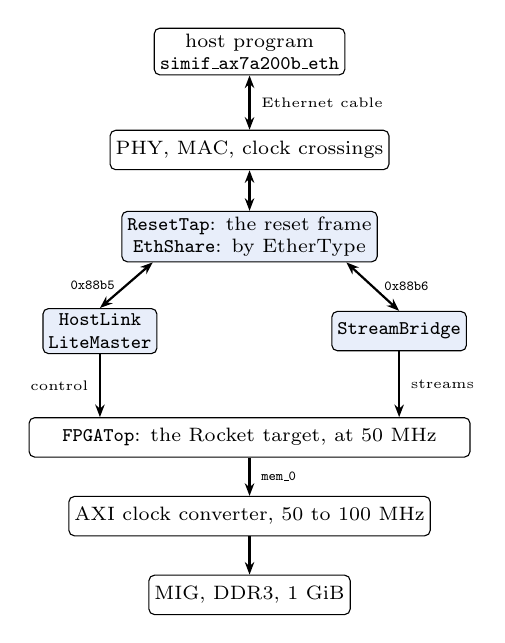
\begin{tikzpicture}
\node[box] (host) at (0, 0) {host program\\\code{simif\_ax7a200b\_eth}};
\node[box] (mac) at (0, -1.25) {PHY, MAC, clock crossings};
\node[art] (share) at (0, -2.35) {\code{ResetTap}: the reset frame\\\code{EthShare}: by EtherType};
\node[art] (ctl) at (-1.9, -3.55) {\code{HostLink}\\\code{LiteMaster}};
\node[art] (str) at (1.9, -3.55) {\code{StreamBridge}};
\node[box, minimum width=56mm] (top) at (0, -4.9) {\code{FPGATop}: the Rocket target, at 50~MHz};
\node[box] (cc) at (0, -5.9) {AXI clock converter, 50 to 100~MHz};
\node[box] (mig) at (0, -6.9) {MIG, DDR3, 1~GiB};
\draw[both] (host) -- node[lbl, right=1mm] {Ethernet cable} (mac);
\draw[both] (mac) -- (share);
\draw[both] (share.south west) ++(4mm, 0) -- node[lbl, left=1mm] {\code{0x88b5}} (ctl.north);
\draw[both] (share.south east) ++(-4mm, 0) -- node[lbl, right=1mm] {\code{0x88b6}} (str.north);
\draw[flow] (ctl.south) -- node[lbl, left=1mm] {control} (ctl.south |- top.north);
\draw[flow] (str.south) -- node[lbl, right=1mm] {streams} (str.south |- top.north);
\draw[flow] (top) -- node[lbl, right=1mm] {\code{mem\_0}} (cc);
\draw[flow] (cc) -- (mig);
\end{tikzpicture}
\caption{FireSim's Rocket design on the AX7A200B. The shaded units are
TxHDL's, lowered as one unit, \code{rocket\_link}.}
\label{fig:f-board}
\end{figure}

The shaded units are lowered together as one unit,
\code{rocket\_link}, so the channels between them are buffered inside
it. Joined by wires in the hand-written top instead, each channel's
valid would depend on its own ready, a combinational loop.
\code{EthShare} reads each frame's EtherType and hands control frames
to \code{HostLink}, whose \code{LiteMaster} performs them on the
control port, and every other frame to \code{StreamBridge}, which
drops those that are not stream frames.
Listing~\ref{lst:f-bridge} is \code{StreamBridge}: \code{StreamLink}
reads and writes the frames, and \code{BeatMaster} performs each
request as an AXI4 burst of one beat. Every unit has a test against a
software model, and the build simulates each lowered netlist against
the same run under \code{nvc} and Verilator.

\streampart{streambridge}{\code{StreamBridge}: the frames on one side,
the 128-bit AXI4 port on the other.}{lst:f-bridge}

The target's DRAM is the board's DDR3, through AMD's MIG~7-series
controller as TxHDL's own designs use it, with one change: its AXI port
is 64 bits wide with 16-bit identifiers, the shape of \code{FPGATop}'s
memory port, and the MIG widens to its 256-bit native port inside. An
AXI clock converter crosses from the simulator's 50~MHz to the MIG's
100~MHz user clock. The simulator, the link and its crossings are held
in reset until the MIG has calibrated.

The reset frame uses that chain. A unit in front of \code{EthShare},
\code{ResetTap}, passes every frame on and raises a reset signal at the
end of a reset frame for this device. It reads frames as they arrive,
so it sees one even while the control master waits on a port that does
not answer. The top then starts the MIG's power-on reset again, and the
MIG's calibration holds the clock converter, the simulator and the link
in reset, as at power-on. The driver sends the frame three times,
since nothing answers it, and the board answers again about 250~ms
later.

Vivado~2025.2 places and routes the design on the
\code{xc7a200tfbg484-2}. It meets timing, with 0.363~ns of setup slack
and 0.036~ns of hold slack, and uses 79\,949 LUTs (60\%), 38\,723
flip-flops (14\%), 202 block-RAM tiles (55\%) and 16 DSPs. The
Nitefury~II's own PCIe build of the same design uses 92\,354 LUTs.

\section{The Host}
\label{sec:f-host}

The host program is FireSim's, from its sources: its main loop, the
bridges' drivers of Chipyard's FireChip, and the design's generated
header from the prebuilt archive. Only the platform file is TxHDL's.
It implements \code{simif\_t}'s register read and write and FireSim's
\code{CPUManagedStreamIO} on two raw sockets, one per EtherType. It
sends each request to every port of the interface cabled to the board,
waits up to 20~ms for the answer, and sends it again up to 50 times.

A raw socket needs the \code{cap\_net\_raw} capability. A binary given
a file capability runs in Linux's secure mode, in which the loader
ignores \code{LD\_LIBRARY\_PATH}, so the driver links Spike, which
FireSim's bridges use, statically. It is one file of 3.7~MB that needs
only the C library's shared objects.

\section{Results}
\label{sec:f-results}

Table~\ref{tab:f-runs} lists the board runs. FireSim's GCD example,
whose bridges are registers only, passed first, on October 27, 2026.
The Rocket design followed the same day. Its driver loaded each program
into the DDR3 through FireSim's TSI bridge, Rocket's boot ROM jumped to
it, and its exit through \code{tohost} ended the run.

\begin{table}[htbp]
\caption{Board runs, October 27 to 29, 2026.}
\label{tab:f-runs}
\centering
\begin{tabular}{@{}lll@{}}
\toprule
Program & What it checks & Result \\
\midrule
GCD & registers & \code{[GCD]PASS} \\
\code{hello.riscv} & DDR3, UART output & passed \\
\code{echo.riscv} & UART input & passed \\
\code{bench.riscv} & speed & 42.5~MHz \\
\code{hello}, TracerV & the stream path & passed \\
\code{hello}, 7 in a row & the reset & passed \\
\bottomrule
\end{tabular}
\end{table}

\code{bench.riscv} times a loop of 50 million iterations with the
core's own counters: 350\,000\,004 instructions in 600\,000\,056 cycles.
The whole run, 639\,520\,037 target cycles, took about 15.03~s of the
host's time on a 50.007~MHz FPGA clock: FireSim reports an effective
target clock of 42.5~MHz, a ratio of 1.18 FPGA cycles per target cycle,
and the driver rounds the time to 15.0~s. That is about 23 million
target instructions per second. An earlier version of this paper gave
45.7~MHz, from a run that followed another on the same simulator and
counted its 48\,114\,360 cycles too. While the target runs on its
own, the link costs nearly nothing: the host steps in only while a
bridge needs it, and this loop needs none.

\code{echo.riscv} echoed a line typed into the driver's standard input,
through FireSim's UART bridge, and stopped at a~\code{q}.

With FireSim's TracerV bridge set to write a trace, \code{hello.riscv}
wrote 399 lines: the boot ROM, the wait while the program loads, and
the program's print loop. The host read them as 1\,596 beats of 16
bytes, four to each 64-byte entry of the stream's queue.

The first attempt, on October 27, wrote an empty trace, and the run
after it got no answer at all. The cause was the missing reset
(issue~2007). Each run writes the simulation's \code{STEP} register
once, and the step never finishes: once the driver exits, the TSI bridge
stops the target until a host serves it. \code{STEP} is a queue that
takes a write only once the step before has finished, so the fourth run
on one simulator waited for ever on its write, and the control path
answered nothing after it. With the reset frame, seven runs in a row
passed with the same cycle count, the traced run among them, and a
board left in that state by the old driver answered again without
reprogramming.

\section{What Is Not Done}
\label{sec:f-not}

\begin{itemize}
\item A fast root file system. Linux 6.18 boots on the Rocket design
from an initramfs since October 30, 2026, and since October 31 with its
root on FireSim's block-device bridge; but every block access is a
register exchange over the cable, and that boot took 132~s against
45.8~s from an initramfs (\texttt{docs/firesim.md}).
\item A bitstream built and released by continuous integration. The
release \texttt{firesim-ax7a200b-rocket-v1} holds the bitstream, the
driver and the programs, cut by hand from one commit
(\texttt{docs/firesim.md}).
\item PCIe. The board stays on its cable for now.
\end{itemize}

\begin{thebibliography}{9}

\bibitem{firesim}
S.~Karandikar \emph{et al.}, ``FireSim: FPGA-accelerated cycle-exact
scale-out system simulation in the public cloud,'' in \emph{Proc.\
ISCA}, 2018.

\bibitem{goldengate}
A.~Magyar \emph{et al.}, ``Golden Gate: Bridging the resource-efficiency
gap between ASICs and FPGA prototypes,'' in \emph{Proc.\ ICCAD}, 2019.

\bibitem{chipyard}
A.~Amid \emph{et al.}, ``Chipyard: Integrated design, simulation, and
implementation framework for custom SoCs,'' \emph{IEEE Micro},
vol.~40, no.~4, 2020.

\bibitem{eth}
F.~Filmar and D.~Janković, ``Ethernet in TxHDL,'' project repository
\code{HDL/txhdl}, \code{//docs:eth}, 2026.

\bibitem{cover}
F.~Filmar and D.~Janković, ``TxHDL documents,'' project repository
\code{HDL/txhdl}, \code{//docs:cover}, 2026.

\end{thebibliography}

\end{document}
